\documentclass[border=10pt]{standalone}
\usepackage[svgnames]{xcolor}
\usepackage{amsmath}
\usepackage{pgfplots}
\pgfplotsset{compat=newest}
\usepackage[sfdefault]{FiraSans}
\usepackage{FiraMono}
\renewcommand*\familydefault{\sfdefault}
\begin{document}
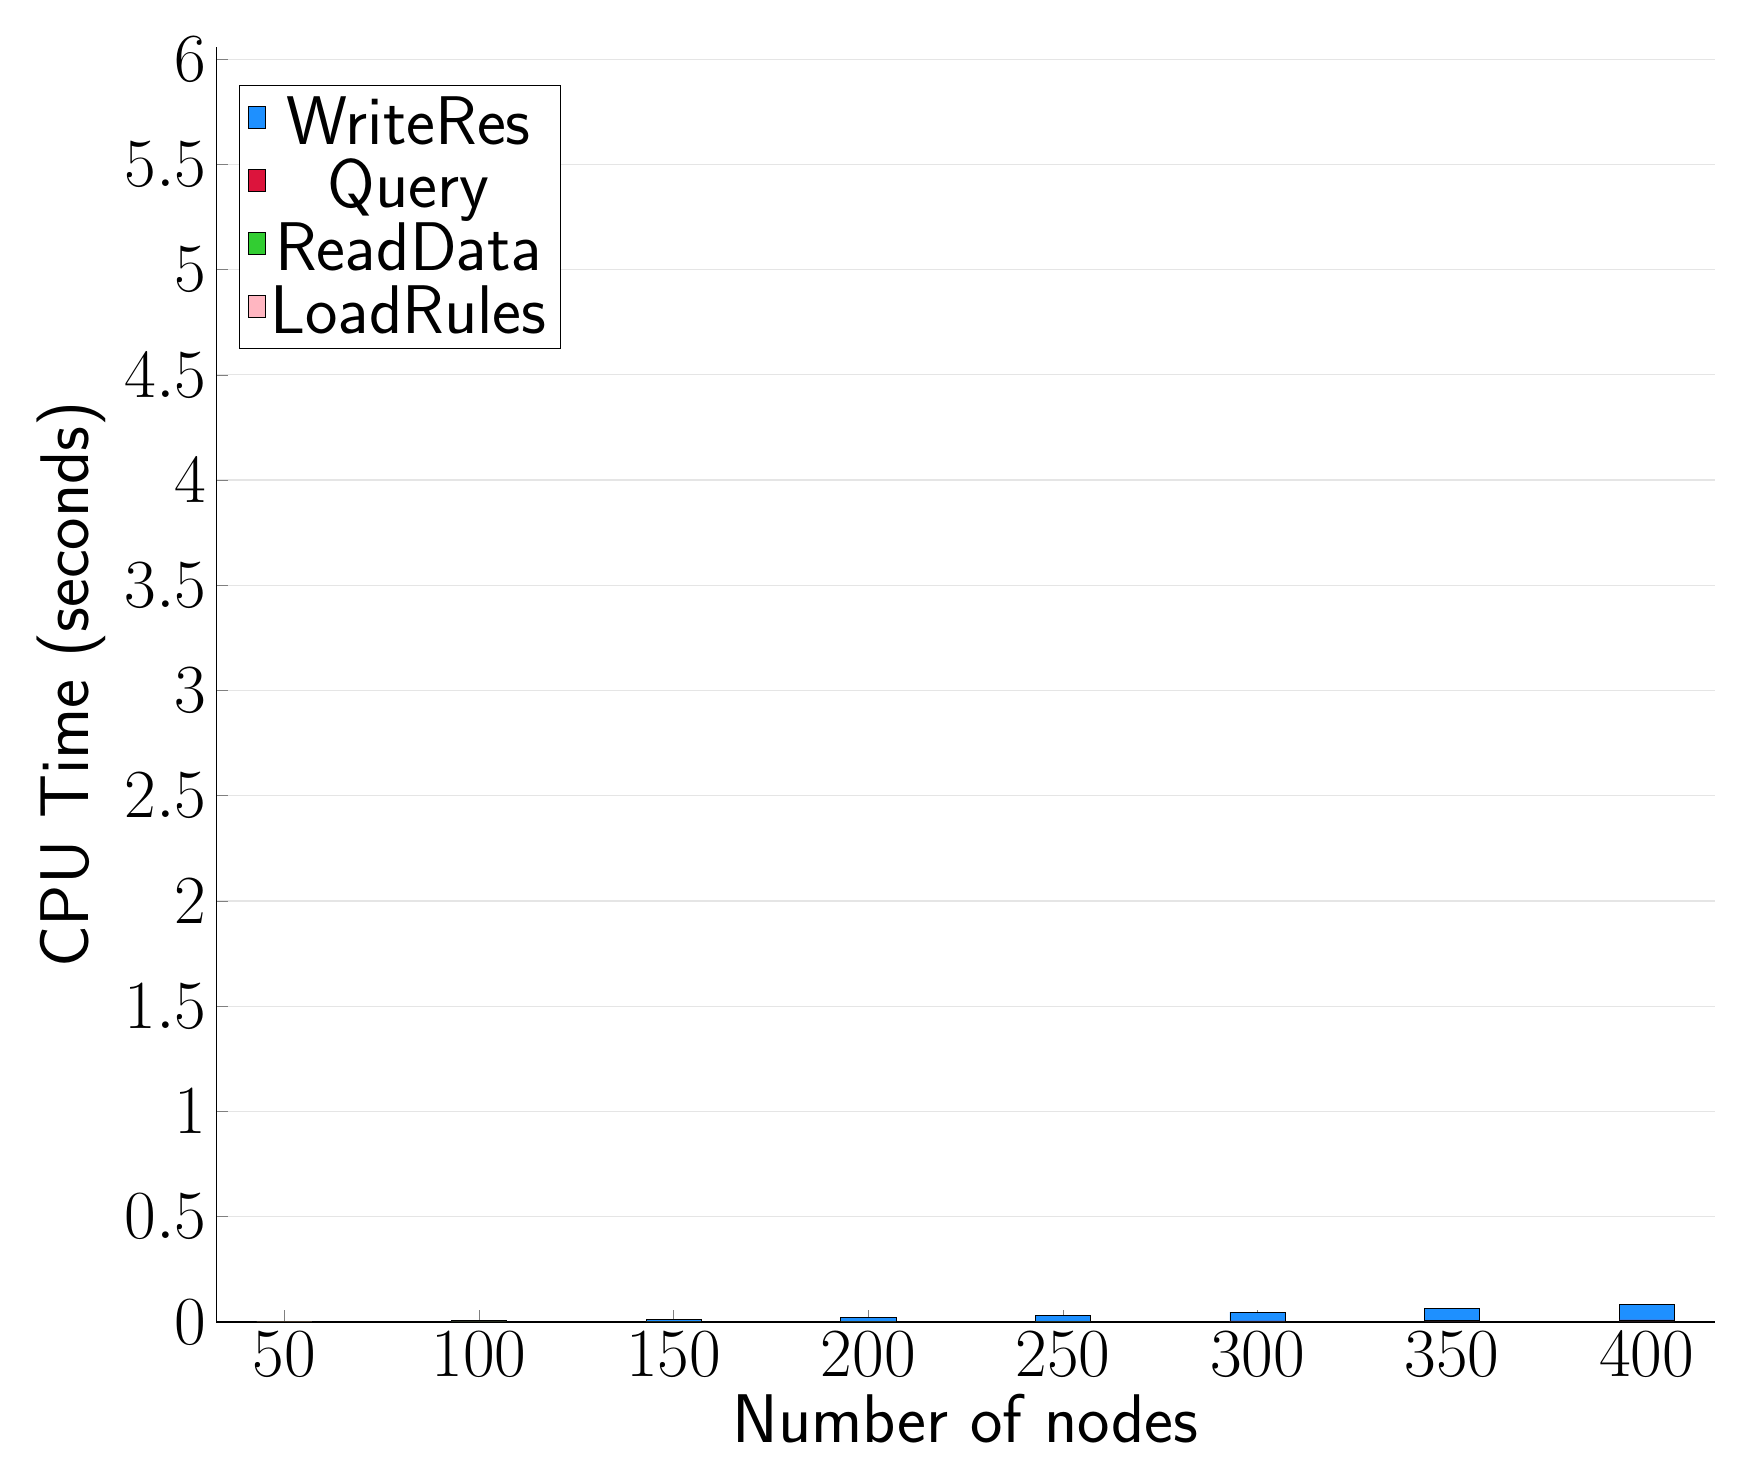
\begin{tikzpicture}
\begin{axis}[
   ybar stacked,
   width=1.7\textwidth,
   bar width=0.7cm,
   ymajorgrids, tick align=inside,
   major grid style={draw=gray!20},
   xtick=data,
   ymin=0, ymax=6.059334,
   axis x line*=bottom,
   axis y line*=left,
   enlarge x limits=0.05,
   legend style={
       at={(0.23, 0.97)},
       anchor=north east,
       legend columns=1,
       font=\Huge,
   },
   ylabel={CPU Time (seconds)},
   xlabel={Number of nodes},
   label style={font=\Huge},
   tick label style={font=\Huge},
]
\addlegendimage{fill=DodgerBlue, draw=black, line width=0.2pt}
\addlegendentry{WriteRes}
\addlegendimage{fill=Crimson, draw=black, line width=0.2pt}
\addlegendentry{Query}
\addlegendimage{fill=LimeGreen, draw=black, line width=0.2pt}
\addlegendentry{ReadData}
\addlegendimage{fill=LightPink, draw=black, line width=0.2pt}
\addlegendentry{LoadRules}
\addplot +[fill=LightPink, draw=black, line width=0.2pt] coordinates {
(50, 0.0006029999999999999)
(100, 0.0006035000000000003)
(150, 0.0006086000000000005)
(200, 0.0006151000000000002)
(250, 0.0005991000000000003)
(300, 0.0006162999999999996)
(350, 0.0006131999999999998)
(400, 0.0006004000000000001)
};
\addplot +[fill=LimeGreen, draw=black, line width=0.2pt] coordinates {
(50, 0.0001740999999999999)
(100, 0.000215)
(150, 0.0002636999999999997)
(200, 0.0003121000000000001)
(250, 0.0003459999999999999)
(300, 0.00039950000000000066)
(350, 0.0004341999999999993)
(400, 0.0004806999999999998)
};
\addplot +[fill=Crimson, draw=black, line width=0.2pt] coordinates {
(50, 0.00012520000000000022)
(100, 0.0004805000000000008)
(150, 0.0010642999999999998)
(200, 0.0018938)
(250, 0.0029652000000000003)
(300, 0.0042975999999999995)
(350, 0.006340799999999999)
(400, 0.008348499999999998)
};
\addplot +[fill=DodgerBlue, draw=black, line width=0.2pt] coordinates {
(50, 0.0011692999999999999)
(100, 0.004517799999999999)
(150, 0.0103823)
(200, 0.0184286)
(250, 0.0288118)
(300, 0.0414263)
(350, 0.056022300000000004)
(400, 0.0739252)
};
\end{axis}
\end{tikzpicture}

\end{document}
